\chapter{Product}

In this chapter we describe the most important tools used during the course of our work. For each section we start with a general description of the software (or framework) purpose and functionalities. After this initial description we provide a more in-depth look regarding some of the more technical aspect of the application. Finally, we describe its relevance in the context of our work.

%********************************** %First Section  **************************************
\section{Dynamics 365 for Finance and Operations / Trade+} 

Dynamics 365 \cite{D365Book} is a cloud-based platform developed by Microsoft Corporation that offers both Enterprise Resource Planning (ERP) and Customer Relationship Management (CRM) solutions. Dynamics 365 for Finance and Operations is an application, part of the Dynamics 365 suite, that offers core ERP functionalities with a particular focus on mid-sized businesses. Said functionalities are: retail, production, supply chain management, procurement (i.e. purchasing), human capital management and finances. The platform can be deployed on-premise, using the company infrastructure, or in the cloud utilizing the Microsoft Azure services. A hybrid deployment is also possible. The platform is accessible with a web-based user interface that replaced the Windows client typical of older versions of the software. Typically customers are obtain the software through certified partners (like Würth Phoenix) that provide the licenses for the software and handle the various implementation related activities such as: development of new features and modification of existing ones, consulting, integration with previously existing infrastructures and system setup. The Dynamics 365 for Finance and Operations source code is composed by multiple \textit{elements} (like classes, tables, forms, menu items, etc.) which are all organized into eight different \textit{layers}. Elements in the lower layers (SYS, FPK, GLS) are handled directly by Microsoft and are related to core functionalities, patches and localization. Middle layers (SLN, ISV) contain elements used by independent software vendors to implement vertical solutions (like Trade+) while higher ones (VAR, CUS, USR) are related to customer specific implementations. Modifications performed in lower layers have an effect on the elements in the higher ones. A group of related elements (all belonging to the same layer) is called a \textit{model} and constitutes a solution (e.g. a warehouse management model). A model is always part of a \textit{package}, which is a compilation/distribution unit formed by one or more models that also contains metadata describing their properties and behaviors. Packages can reference each other and can be combined to form a \textit{deployable package}, a deployable unit that can be applied to an instance of the D365 software. In Dynamics 365 for Finance and Operations we identify three data types: Setup data (specifies the underlying structure of the business and is almost never changed), master data (describes entities such as products and customers and is rarely changed) and transaction data (describes all the activities performed by the company and is constantly updated). The Architecture \cite{D365Book2} of Dynamics 365 for Finance and Operations can be seen as list seven conceptual components:

\begin{itemize}
    \item \textbf{Identity}. The authentication process and access control are managed by the Azure Active Directory, a cloud-based application capable of synchronizing with both on-premise directories and online services. In a cloud deployment of D365, AD uses the Security Assertion Markup Language 2.0 to securely exchange information between parties. Authentication in on-premise iterations of D365 is handled by the Active Directory Federation Services.
    
    \item \textbf{Storage}. A primary database handles the bulk of the read and write workload. This includes most of the primary transactions, the import/export of files, the financial reporting and the handling of stored documents. Some of the read-only interactions are redirected to a secondary database. A third read-only database handles the business analytics related activities. SQL Azure is used on cloud deployments while Microsoft SQL Server 2016 is utilized in on-premise ones.
    
    \item \textbf{Platform}. Dynamics 365 for Finance and Operations provides its functionalities through different applications (Application Object Servers, Retail Servers, Management Reporter and SQL Server Reporting Services) that are all hosted and run on Azure Compute Virtual Machines in cloud deployments or on Microsoft Service Fabric Standalone Clusters in on-premise ones. The platform layer includes all the resources needed to perform this hosting process. 
    
    \item \textbf{Application}. The application components, code and metadata are the same for all deployment types. The application stack is divided into three models: Application Platform (which is the lower model that contains the code that handles the core application features such as runtime, data access, SQL Server Reporting Services, task recording, data import/export, batch and mobile frameworks), Application Foundation (containing shared code used by multiple application modules) and Application Suite (that represents the top level code that provides the basic functionalities that can be expanded or modified by Microsoft Partners). The application runtime is handled by the Application Object Server which manages connection between clients and database and enforces security. AOS is a ASP.NET web application that contains all the kernel components (security and data access information, forms engine, metadata, UI interaction services, etc.) needed to interact with the application.
        
    \item \textbf{Client}. The Dynamics 365 GUI is provided by the HTML 5 browsers-based client and the mobile applications. Both alternatives also integrate features from the Office 365 suite.
    
    \item \textbf{Development tools}. Visual Studio is the development environment used to extend or modify the application. The first step in customizing Dynamics 365 for Finance and Operations (by adding new code and functionalities) is the creation of a new model that can be deployed in its own package (Extension) or as a part of an existing one (Overlayering).
    
    \textit{Overlayering} means copying the elements of an existing model into a newly created one that can be modified by the developer. This new model must reside on a higher layer and belong to the same package as the original one. When the application is executed only the code contained in the copy (residing higher up in the layer hierarchy) is considered. The peculiarity of this technique resides in the fact that effectively all the model code is duplicated (not only the one that is modified or added by the developer), hence potentially creating a big overhead. Modifying via \textit{Extension} means generating a new model in order to add functionalities to an existing one (i.e. extend) without creating an entire copy of it. The new model (that, unlike overlayering, resides in his own package) is created together with one or more references to the existing models that need to be expanded. This references allow the new model to expand and interact with the elements of the referenced ones (e.g. accessing a table, calling a class, etc.) without directly modifying their source code. Untouched source code means shorter compilation times and decreased likelihood of issues when the application is updated. Customizations are always handled inside a \textit{project}, which is a logical construct that helps a developer manage the interested elements. A project may only contain elements coming from a single model. Developers work on the application using DEV VMs, which are machines pre-configured with Visual Studio, Dynamics, and SQL servers. An additional machine is needed to take the developed code, perform the build operations, execute tests and create the deployable packages.
    
    \item \textbf{Lifecycle Services}. The implementation activities can be facilitated with the use of Lifecycle Services, a collaborative workspace used to define and share standardized processes across the company in order to improve the predictability of the implementation process.
\end{itemize}

As stated before Dynamics 365 for Finance and Operations represents a general approach to ERP and it's not generally meant to be sold directly to customers without undergoing at least some degree of personalization. A personalized version of the software is called a \textit{vertical}. Trade+ is the vertical solution offered by Würth Phoenix that focuses on enhancing the wholesale and distribution capabilities of the base offering. The main features offered by Trade+ are related to: 
Sales \& Marketing (administration of associations and groups, back order processing, extended pricing, pricing administration, extended information in the order location, automatic e-mail dispatch), Purchasing \& disposition (automatic forecast calculation, extended ABC classification, determination of average monthly requirements, dunning for suppliers, supplier evaluation, article discontinuation control), Warehouse management \& logistics (Extended storage and retrieval strategies, preventive and urgent stock transfers, mobile solution for warehouse management, route management and route planning, label printing) and Business Intelligence \& Reporting (Data Warehouse, Data Cubes and Reports for Trading and Production Companies).
On top of this features the application also provides various customizations on existing functionalities that present added or modified details and user interface element in comparison to the version provided by Microsoft. This fact brought us to choose five business processes that, despite being already present in the base application, could be affected in some ways by the mentioned changes and extensions provided by the company.

%********************************** %Second Section  **************************************
\section{Team Foundation Server / Azure DevOps} 

Azure DevOps \cite{DevOps} (previously known as Visual Studio Team Services) is a lifecycle management tool developed by Microsoft. Just like Dynamics 365 this tool can exist on the cloud, as Azure DevOps, or on-premise, as Team Foundation Server (from 2019 onward this version will be renamed Azure DevOps Server). The architectural difference between the two iteration of the software goes beyond the scope of this chapter given the fact that both versions offer the same set of functionalities to the end user. For the sake of simplicity from now on we will refer to the application as Azure DevOps. Azure DevOps is composed by five elements, each covering a different aspect of the lifecycle management process [Figure \ref{fig:devOpsDevelopment}]:

\begin{itemize}
    \item \textbf{Boards} offers a way to plan and track all the work activities related to development (epics, features and user stories), testing (test plans, test suites and test cases) and bug fixing. Each item is assigned to one or more team members and comes with various information such as: title, description, effort estimate, relation to other elements, etc. The visualization, tracking and modification of the status (new, active, resolved, closed, removed) of each item can be performed using a backlog or a Kanban board. Sprint management is also supported.
    \item \textbf{Repos} is a set of version control features that developers can use to track code changes, branch, fork and create pull requests. Azure Repos supports both Git (as a distributed VC) and Team Foundation Version Control (as a centralized VC) and can be connected with various development environments. Using Git every developer saves a full copy of the repository on the machine and is able to work on it even when disconnected from the network. With TFVC only one iteration of the project is saved locally, all other data is maintained on the server.
    \item \textbf{Pipelines} takes the code from Repos (or any other supported providers like GitHub) and enforces Continuous Integration and Continuous Delivery techniques by performing automated sequence of steps (called pipelines) to build, test and deploy the newly written code. The execution of each pipelines can be scheduled following specific trigger events (e.g. code changes are checked in) and their execution can be monitored directly from the environment.
    \item \textbf{Test Plans} allows developers to perform automated, manual and load testing techniques and to monitor the status of each test case and test plan for a specific project. Issues during test execution are notified to all team member and can be further documented with additional information. Naturally the elements of Azure Test Plans can be associated with the previously mentioned pipelines.
    \item \textbf{Artifacts} allows the management of (NuGet, npm and Maven) packages.
\end{itemize}

\begin{figure}[ht]
	\centering
	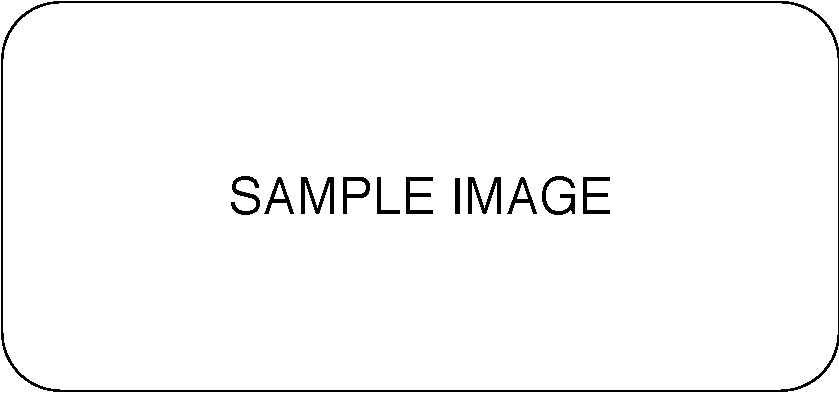
\includegraphics[scale=0.7]{Images/SampleImage.pdf}
	\caption{Development using Azure DevOps}
	\label{fig:devOpsDevelopment}
\end{figure}

The application is normally accessed via the web-based client but its functionalities can also be integrated directly into the development environment with the Visual Studio Team Explorer plug-in. Once connected to a project the developer can see his assigned work items, manage his pending changes (i.e. modifications to the code that have yet to be checked in), explore and interact with version control and manage builds related to his code changes. Of particular importance for our work is how Azure DevOps helps developers plan, develop, monitor and integrate test cases for a given project in order to easily implement CI/CD techniques.

%********************************** %Third Section  **************************************
\section{SysTest Framework} 

The SysTest framework provides developers a set of classes and methods that can be utilized to author test cases. In general (for ERP application) we identify five kind of testing techniques: unit testing (SysTest), feature/component testing (SysTest + Task recorder), integration testing (SysTest + Task recorder), performance testing (PerfSDK), acceptance testing (Task recorder) and regression testing (SysTest + DevOps).  The first step in creating a test case is extending the interested class with \textit{SysTestCase}. Every test class should be named after the component/feature/process that is being tested and may contain one or more test methods. Test methods are \textit{void} and are recognized by the system via the decorator reference to the \textit{SysTestMethodAttribute} class. As a best practice the level of granularity of the test method should also be stated via the \textit{SysTestGranularityAttribute} class. As a general rule a test method should be organized into three sections:

\begin{itemize}
    \item \textbf{Arrange}. The data used during the test is declared and, if needed, inserted into the database. This declaration phase should be kept minimal (i.e. declare only data that is strictly needed in order to make the test case run) and can be skipped altogether in certain scenarios.
    \item \textbf{Act}. The testing operation are executed.
    \item \textbf{Assert}. The results of the act block are observed and validated. The assert statement is an essential part of a test method because it determines the nature of the outcome (successful or unsuccessful) once the test is executed. In order to perform an assert statement the \textit{this} keyword is used (since the \textit{SysTestCase} class extends the \textit{SysTestAssert} one) followed by one of the assert methods (assertEquals, assertTrue, assertNotNull, etc.).
\end{itemize}

As mentioned before it is also possible to generate coded test cases directly from XML recordings obtained through the Task recorder. Although a more in-depth look at this tool will be provided in the next chapter, it is important to describe how the tests generated from this process differ from the ones described above. 
A newly generated test is composed by: a variable declaration area, a \textit{void SetUpTestCase} method that prepares the environment, a \textit{void setupData} method that assigns values to the previously defined variables and a single \textit{void testMethod}. The peculiarity of this \textit{testMethod} resides in the fact that it uses \textit{Form Adaptors} in order to simulate interactions with a Dynamics 365 for Finance and Operations GUI. We move in the application using this wrapper classes that provide an API that mimics possible user interaction with the system elements. This allows the creation of test cases in which the actions taken during the recording process by a user are translated into X++ code. Because of this reason test cases generated from task recordings are considered \textit{headless}, this means that they are able to mimic a GUI interactions without actually having to display it. Another peculiarity of this method is the fact that it does not contain an assert section. Because of this reason a generated test case is considered successful when all the steps can be completed without raising any errors.
Another relevant topic related to the the SysTest framework is how it handles the creation, deletion or modification of data during test execution. For Dynamics 365 the objective was to allow developer to execute any test case without the risk of compromising the state of the underlying database. This meant returning to the DB original state at the end of every test(s) execution. In order to implement this feature a rollback mechanism [Figure \ref{fig:SysTestRollback}] was baked into the framework. This was achieved by treating each execution as a single DB transaction and by utilizing SQL SavePoints to implement nested/sub transactions. Because of this reason a savepoint is created (by a savepoint manager) every time the framework, a test suite, a test class or a test method are started. When one of this elements completes its execution, the data is restored to the previous savepoint, effectively nullifying the changes that have been performed up to that point. It is important to note that the rollback mechanism always follow the hierarchy of the transaction (e.g. when a test method is completed, the framework goes back to the savepoint created immediately before the start of the method). The implementation of this technique ensures that DB is not left in an unreliable state after the execution process.

\begin{figure}[ht]
	\centering
	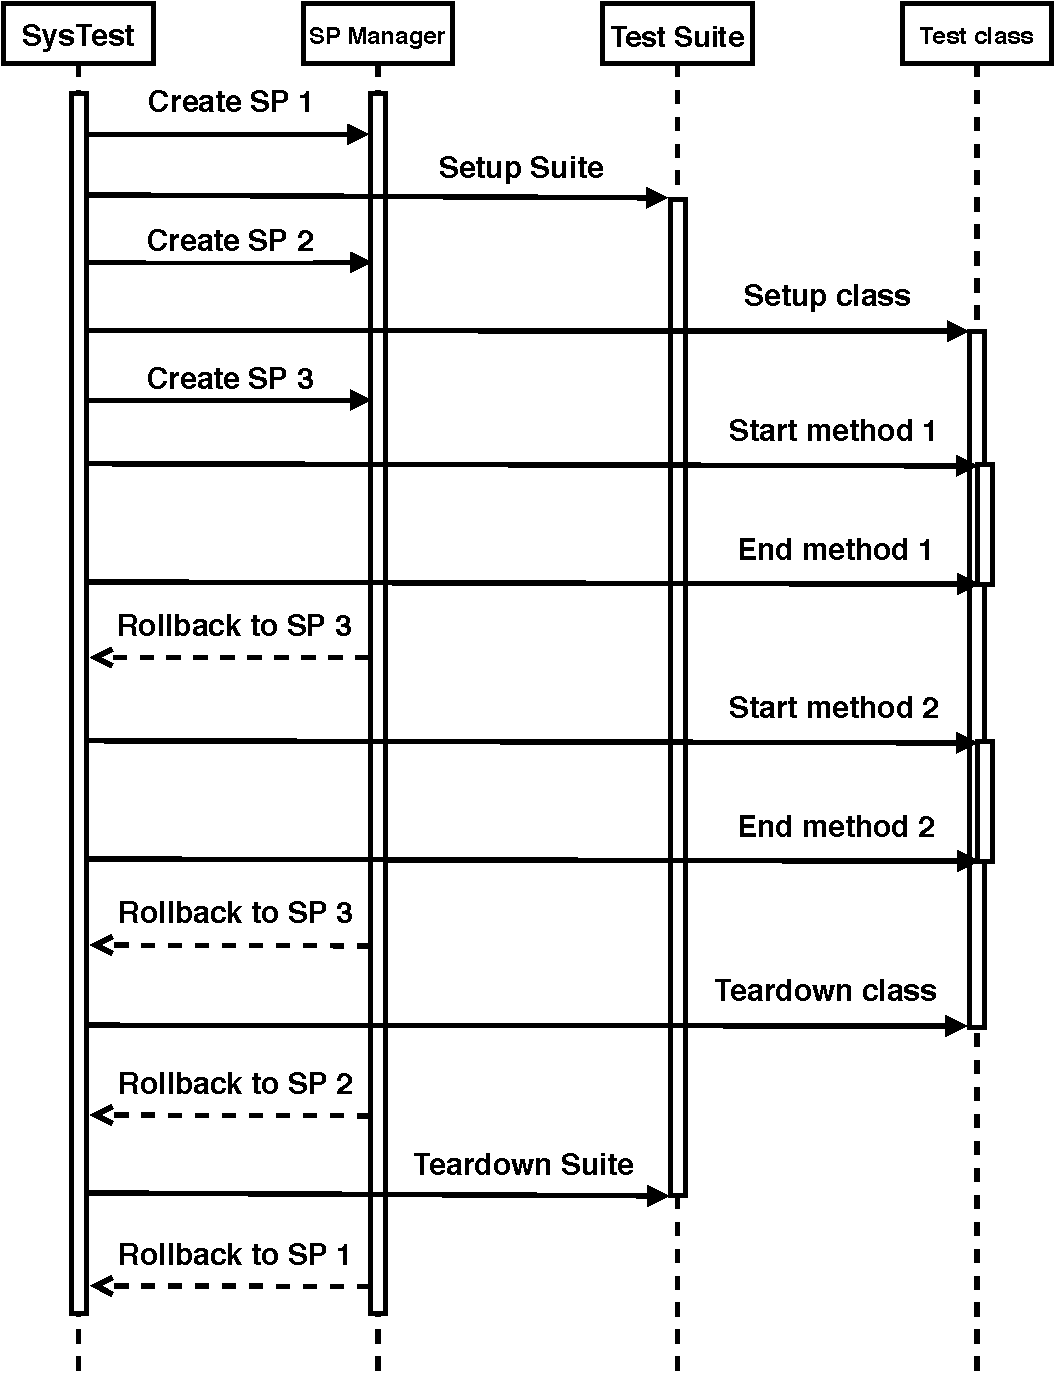
\includegraphics[scale=0.6]{Images/SysTestRollback.pdf}
	\caption{SysTest Framework rollback (Class and method)}
	\label{fig:SysTestRollback}
\end{figure}

DESCRIBE RELEVANCE IN CONTEXT OF WORK HERE
